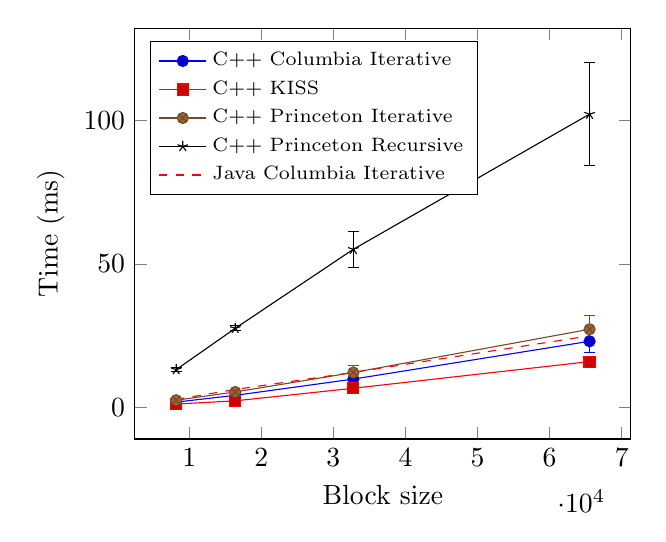
\begin{tikzpicture}
\begin{axis}[xlabel={Block size},ylabel={Time (ms)},width=0.65\linewidth,legend pos=north west,scaled y ticks = false,legend cell align=left,legend style={font=\scriptsize}]
\addplot+[error bars/.cd, y dir=both,y explicit] coordinates {
(8192, 1.9326) +- (0.2654, 0.2654)
(16384, 4.2789) +- (0.6399, 0.6399)
(32768, 9.9388) +- (1.6341, 1.6341)
(65536, 23.1031) +- (3.9019, 3.9019)
};
\addplot+[error bars/.cd, y dir=both,y explicit] coordinates {
(8192, 1.2470) +- (0.2301, 0.2301)
(16384, 2.3713) +- (0.4915, 0.4915)
(32768, 6.7420) +- (1.2931, 1.2931)
(65536, 16.0281) +- (1.8073, 1.8073)
};
\addplot+[error bars/.cd, y dir=both,y explicit] coordinates {
(8192, 2.5845) +- (0.2085, 0.2085)
(16384, 5.4518) +- (0.5858, 0.5858)
(32768, 12.2266) +- (2.4651, 2.4651)
(65536, 27.2805) +- (4.8616, 4.8616)
};
\addplot+[error bars/.cd, y dir=both,y explicit] coordinates {
(8192, 13.2345) +- (0.7311, 0.7311)
(16384, 27.6080) +- (0.9098, 0.9098)
(32768, 55.1227) +- (6.2636, 6.2636)
(65536, 102.1585) +- (17.9911, 17.9911)
};
\addplot+[style=dashed,color=red,mark=none] coordinates {
(8192, 2.8726) +- (0.3247, 0.3247)
(16384, 6.3214) +- (1.0542, 1.0542)
(32768, 12.2634) +- (2.9076, 2.9076)
(65536, 24.9874) +- (4.6266, 4.6266)
};
\legend{C++ Columbia Iterative , C++ KISS , C++ Princeton Iterative , C++ Princeton Recursive, Java Columbia Iterative}
\end{axis}
\end{tikzpicture}
